\begin{frame}{Recent theoritial status}
  D. Jido et el. suggested tow pole state, $\bar{K}N$(higher) and $\pi \Sigma$(lower). \\
  \hspace{25mm} {\scriptsize Nucl. Phys. A 725, 181 (2003). }\\
  \hspace{20mm} $\Rightarrow$ Similar method and result were come out.
  \vspace{3mm} \\
  
  \begin{tabular}{cc}
    \begin{minipage}{0.5\hsize}
      \begin{figure}
        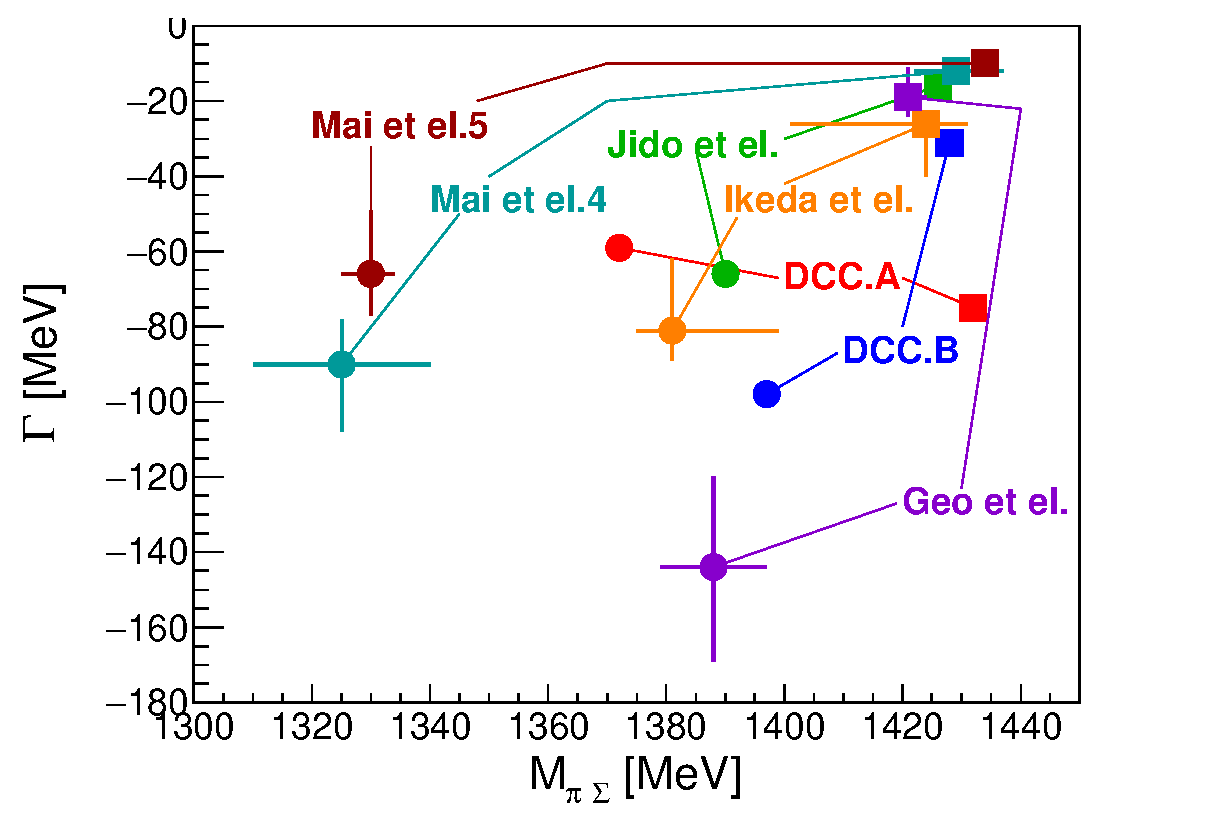
\includegraphics[width=6cm]{../pic/Dron/L1405_pole_wFit.eps}
      \end{figure}
    \end{minipage}
    
    \begin{minipage}{0.5\hsize}
      NLO w/ Constraint by SHIDDARTA.\\ 
      \hspace{3mm} Y. Ikeda, et el., \\
      \hspace{6mm} {\scriptsize Nucl. Phys. A {\bf 881}, 98 (2012)} \\
      \hspace{3mm} Z.-H. Guo and J. Oller, \\
      \hspace{6mm} {\scriptsize Phys. Rev. C {\bf 87}, 3, 035202 (2013)}\\
      Filltering by CLAS data \\
      \hspace{3mm} M. Mai and U.-G. Mei$\beta$ner \\
      \hspace{6mm} {\scriptsize Eur. Phys. J. A {\bf 51}, 3, 30}\\
      DCC method \\
      \hspace{3mm} H. Kamano et el.\\
      \hspace{6mm} {\scriptsize Phys. Rev. C{\bf 92}, 025205 (2015)}
    \end{minipage}
  \end{tabular}
\end{frame}
